\hypertarget{randomF77_8c}{
\section{random\-F77.c File Reference}
\label{randomF77_8c}\index{randomF77.c@{randomF77.c}}
}
{\tt \#include \char`\"{}party.h\char`\"{}}\par


Include dependency graph for random\-F77.c:\begin{figure}[H]
\begin{center}
\leavevmode
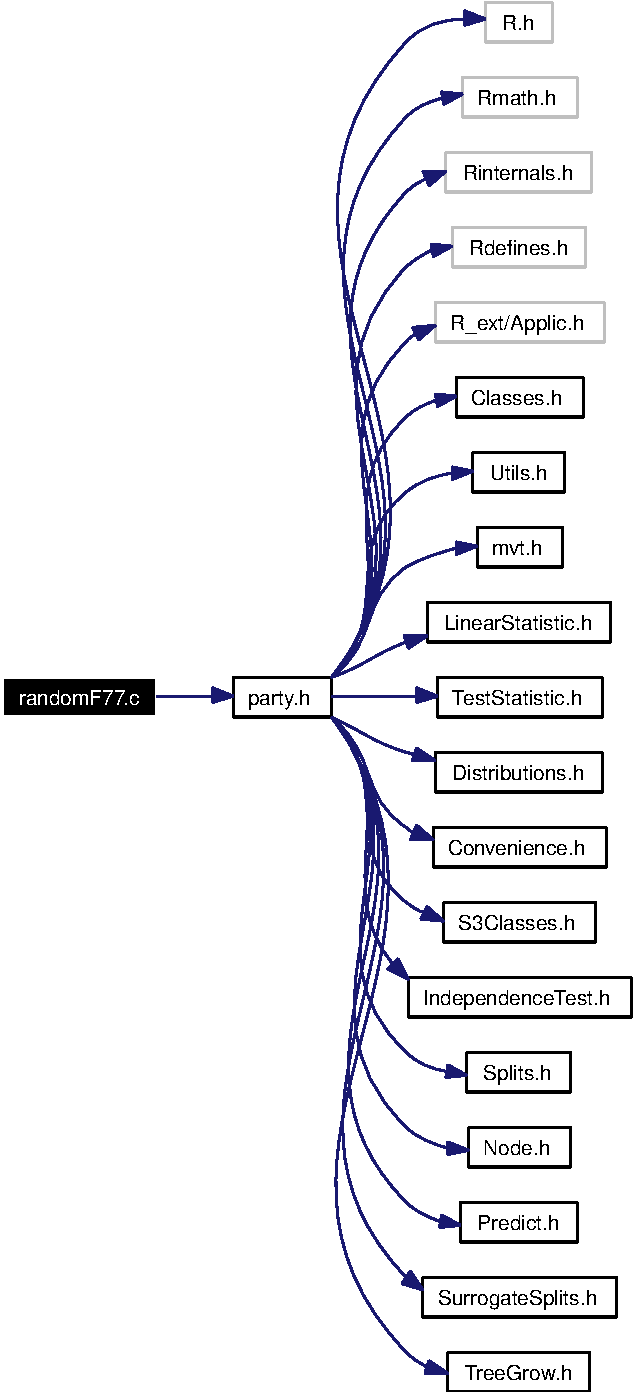
\includegraphics[width=171pt]{randomF77_8c__incl}
\end{center}
\end{figure}
\subsection*{Variables}
\begin{CompactItemize}
\item 
void F77\_\-SUB( \hyperlink{randomF77_8c_a0}{rndstart} )(void)
\item 
void F77\_\-SUB( \hyperlink{randomF77_8c_a1}{rndend} )(void)
\item 
double F77\_\-SUB( \hyperlink{randomF77_8c_a2}{unifrnd} )(void)
\end{CompactItemize}


\subsection{Variable Documentation}
\hypertarget{randomF77_8c_a1}{
\index{randomF77.c@{random\-F77.c}!rndend@{rndend}}
\index{rndend@{rndend}!randomF77.c@{random\-F77.c}}
\subsubsection[rndend]{\setlength{\rightskip}{0pt plus 5cm}void F77\_\-SUB( \hyperlink{randomF77_8c_a1}{rndend})(void)}}
\label{randomF77_8c_a1}




Definition at line 12 of file random\-F77.c.\hypertarget{randomF77_8c_a0}{
\index{randomF77.c@{random\-F77.c}!rndstart@{rndstart}}
\index{rndstart@{rndstart}!randomF77.c@{random\-F77.c}}
\subsubsection[rndstart]{\setlength{\rightskip}{0pt plus 5cm}void F77\_\-SUB( \hyperlink{randomF77_8c_a0}{rndstart})(void)}}
\label{randomF77_8c_a0}




Definition at line 11 of file random\-F77.c.\hypertarget{randomF77_8c_a2}{
\index{randomF77.c@{random\-F77.c}!unifrnd@{unifrnd}}
\index{unifrnd@{unifrnd}!randomF77.c@{random\-F77.c}}
\subsubsection[unifrnd]{\setlength{\rightskip}{0pt plus 5cm}double F77\_\-SUB( \hyperlink{randomF77_8c_a2}{unifrnd})(void)}}
\label{randomF77_8c_a2}




Definition at line 13 of file random\-F77.c.